\documentclass{beamer}

\usepackage{helvet}
\usepackage{hyperref, graphicx}
\usepackage{amsthm}
\usepackage{etoolbox}

\usetheme{default}
\setbeamertemplate{navigation symbols}{}
\AtBeginSection[ ]
{
\begin{frame}{Outline}
    \tableofcontents[currentsection]
\end{frame}
}

% Default fixed font does not support bold face
\DeclareFixedFont{\ttb}{T1}{txtt}{bx}{n}{11} % for bold
\DeclareFixedFont{\ttm}{T1}{txtt}{m}{n}{12}  % for normal - use in headings

% Custom colors
\usepackage{color}
\definecolor{TUGray}{RGB}{101,101,137}
\definecolor{TUBlack}{RGB}{30,0,0}
\definecolor{mygreen}{RGB}{45,111,63}
\definecolor{keywords}{RGB}{205,114,0}
\definecolor{comments}{RGB}{181,51,139}
\definecolor{strings}{RGB}{58,144,81}
\definecolor{numeric}{RGB}{66,110,176}
\definecolor{linos}{rgb}{0.4,0.4,0.4}
\definecolor{links}{rgb}{0,0.4,0.75}

\definecolor{bggray}{RGB}{232, 233, 235}

\usecolortheme[named=mygreen]{structure}
\setbeamercolor{normal text}{fg=TUBlack}\usebeamercolor*{normal text}

\setbeamercolor{codecol}{fg=TUGray!25!black,bg=bggray}

\hypersetup{colorlinks, linkcolor=links, urlcolor=links}

\usepackage[T1]{fontenc}
\usepackage[sfdefault,scaled=.85]{FiraSans}
\usepackage{newtxsf}

\usepackage{listings}

\newtoggle{InString}{}% Keep track of if we are within a string
\togglefalse{InString}% Assume not initally in string

\newcommand\digitstyle{\color{numeric}}
\makeatletter
\newcommand{\ProcessDigit}[1]
{%
  \ifnum\lst@mode=\lst@Pmode\relax%
   {\digitstyle #1}%
  \else
    #1%
  \fi
}
\makeatother

\lstset{literate=%
    {0}{{{\ProcessDigit{0}}}}1
    {1}{{{\ProcessDigit{1}}}}1
    {2}{{{\ProcessDigit{2}}}}1
    {3}{{{\ProcessDigit{3}}}}1
    {4}{{{\ProcessDigit{4}}}}1
    {5}{{{\ProcessDigit{5}}}}1
    {6}{{{\ProcessDigit{6}}}}1
    {7}{{{\ProcessDigit{7}}}}1
    {8}{{{\ProcessDigit{8}}}}1
    {9}{{{\ProcessDigit{9}}}}1
	{<=}{{\(\leq\)}}1
	{>=}{{\(\geq\)}}1,
	% morestring=[b]",
    % morestring=[b]',
    % morecomment=[l]//,
}

% Python style for highlighting
\newcommand\pythonstyle{\lstset{
language=Python,
basicstyle=\ttfamily\tiny,
numbers=left,
numberstyle=\tiny\color{linos},
morekeywords={self},              % Add keywords here
keywordstyle=\tiny\color{keywords},
commentstyle=\it\tiny\color{comments},    % Custom highlighting style
stringstyle=\tiny\color{strings},
xleftmargin=18pt,
xrightmargin=4pt,
aboveskip=0pt,
belowskip=0pt,
escapeinside={(*@}{@*)},
frame=l,                         % Any extra options here
showstringspaces=false,
keepspaces=true
}}

% Python environment 
\lstnewenvironment{python}[1][]
{
	\pythonstyle
	\lstset{
	#1
	}
}
{}

% wrap the Python environment
\newenvironment{codeblock}
    {\hfill\begin{beamerboxesrounded}[lower=codecol, width=0.8\textwidth]
    \medskip

    }
    { 
    \end{beamerboxesrounded}\hfill
    }

\theoremstyle{example}
\newtheorem{question}{Question}

\newcommand{\ct}[1]{\lstinline[language=Python]!#1!}
\newcommand{\ttt}[1]{{\small\texttt{#1}}}
\newcommand{\lsitem}[2]{\ttt{{#1}[}\ct{#2}\ttt{]}}

\author{Chris Cornwell}
\date{Feb 4, 2025}
\title{The Random package, Defining Custom Functions}

\begin{document}

\begin{frame}
\titlepage
\end{frame}

\begin{frame}
\frametitle{Outline}
\tableofcontents
\end{frame}

\section{Random functions in NumPy}

%%%%
\begin{frame}[fragile]
\frametitle{The {\ttm random} submodule in NumPy}
From documentation: Within NumPy is the submodule \ttt{random} which ``implments pseudo-random number generators\ldots with the ability to draw samples from a variety of probability distributions.''
%\pause
\begin{enumerate}
    \item Uniform discrete: to sample \ttt{m} numbers from the uniform distribution on the integers in \ttt{range(n)}, use the function \ttt{np.random.randint(n, size=m)}. 
    \begin{itemize}
        \item An optional additional integer in the arguments: give a lower bound.\footnote{The default lower end is 0, to sample between 0 and \ttt{n-1}.}
        \item If size argument not given, just one number returned. If the \ttt{size=m} is given, returns a NumPy array.
    \end{itemize}
\end{enumerate}

%\pause 
\begin{codeblock}

\begin{python}
    # 20 integers, each equally likely, between 1 and 10
    np.random.randint(1, 11, size=20)
\end{python}

\end{codeblock}

%\pause
\begin{enumerate}
    \item[] Commands above will sample with replacement.
    \begin{itemize}
        \item To sample without replacement, use argument \ttt{replace=}{\color{numeric}\ttt{False}}.
    \end{itemize}
\end{enumerate}

\end{frame}

%%%%
\begin{frame}[fragile]
\frametitle{The {\ttm random} submodule in NumPy}

\begin{enumerate}
    \setcounter{enumi}{1}
    \item Uniform continuous: to sample \ttt{m} floats in the interval \ttt{[a, b)}, use the function \ttt{np.random.uniform(a, b, size=m)}.
    \begin{itemize}
        %\pause
        \item The defaults for the left \& right endpoints are 0 and 1. This means that \ttt{np.random.uniform(size=m)} will sample from the unit interval.
        \item An alternative: \ttt{np.random.random(size=m)}. Only samples from the unit interval, but, can get samples from \ttt{[a,b)} by multiplying and adding (below).
    \end{itemize}
\end{enumerate}

\vspace*{12pt}
%\pause
\begin{codeblock}

\begin{python}[numbers=none]
(b-a)*np.random.random(size=m) + a
\end{python}

\end{codeblock}

\end{frame}

%%%%
\begin{frame}[fragile]
    \frametitle{The {\ttm random} submodule in NumPy}
    
    \begin{enumerate}
        \setcounter{enumi}{1}
        \item Uniform continuous: to sample \ttt{m} floats in the interval \ttt{[a, b)}, use the function \ttt{np.random.uniform(a, b, size=m)}.
        \item Normal distribution: to sample \ttt{m} floats from the normal distribution, with mean \ttt{mu} and standard deviation \ttt{sigma}, use the function \ttt{np.random.normal(mu, sigma, size=m)}
        \begin{itemize}
            \item The two arguments for the mean and standard deviation have default 0 and 1, respectively.
            \item Not uncommon to use the \emph{keywords} for these arguments,\footnote{Using keyword makes the argument not \emph{positional} anymore; arguments coming after it must have keyword too.} as in 
            \begin{center}\ttt{np.random.normal(loc=mu, scale=sigma, size=m)}\end{center}
        \end{itemize}
    \end{enumerate}

    %\pause
    Larger the sample, the closer the distribution of that sample (i.e., normalized histogram) should be to the theoretical pdf. Can we display this in a plot?
\end{frame}
    
%%%%
\begin{frame}[fragile]
\frametitle{Visualizing the distribution}
Using uniform distribution on interval $[a,b)$: for subinterval of width $\delta$, probability $\delta\frac{1}{b-a}$ of getting a sample in that interval.

%\pause
Consequence: plot (normalized) histogram of sample over $[a,b]$; \emph{close} to the distribution means bars are close to height $1/(b-a)$.\newline 
Below: sample of size 50, from \ttt{uniform(0, 5)}.

\begin{codeblock}

\begin{python}
xx = np.linspace(0,5)
sample = np.random.uniform(0, 5, size=50)
# will also plot horizontal line at height 1/(b-a)
plt.plot(xx, [1/5]*len(xx), color='black')
plt.hist(sample, bins=10, density=True)
plt.show()
\end{python}

\end{codeblock}

%\pause
\centering
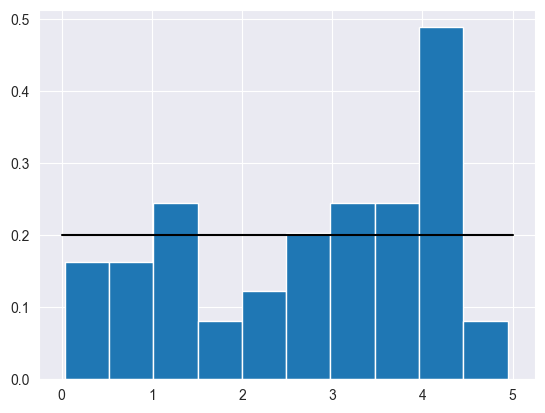
\includegraphics[height=0.35\textheight]{histogram_of_sample1.png}

\end{frame}

%%%%
\begin{frame}[fragile]
\frametitle{Visualizing the distribution}

A larger sample size will (on average) give a distribution that is closer to the \emph{true} one. For example, by changing our previous code so that the sample size is 5000, we can see the sample distribution get much closer.

%\pause
\centering
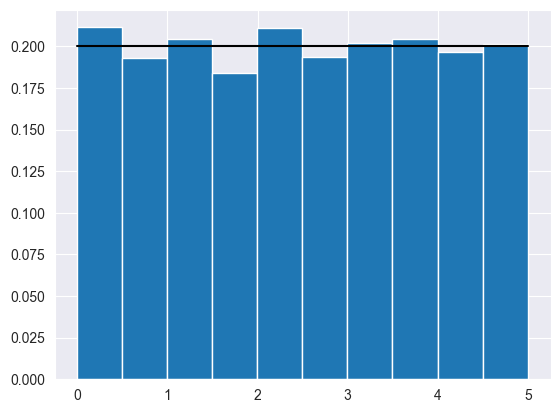
\includegraphics[height=0.4\textheight]{histogram_of_sample2.png}

\end{frame}

%%%%
\begin{frame}[fragile]
\frametitle{Visualizing the normal distribution}
Using the normal distribution, mean $\mu$ and std.deviation $\sigma$, the density function is 
\[{\scriptsize 
p(x) = \frac{1}{\sqrt{2\pi\sigma^2}}e^{-\frac{(x-\mu)^2}{2\sigma^2}}.
}\]

Below is a normalized histogram of a sample of size 100.\footnote{Doubled the sample size and the number of bins, due to greater variability in the pdf of the distribution.}

%\pause

% \begin{codeblock}

% \begin{python}
% xx = np.linspace(-3,3)
% sample = np.random.normal(0, 1, size=100)
% plt.hist(sample, bins=20, density=True)
% plt.show()
% \end{python}

% \end{codeblock}

%\pause
\centering
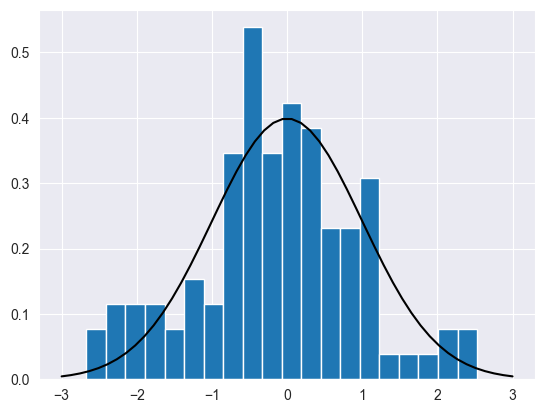
\includegraphics[width=0.4\textwidth]{histogram_of_sample3.png}

\end{frame}

%%%%

\begin{frame}[fragile]
\frametitle{Visualizing the normal distribution}
    
A larger sample size gives a distribution that is closer to the bell curve.
    
%\pause
\centering
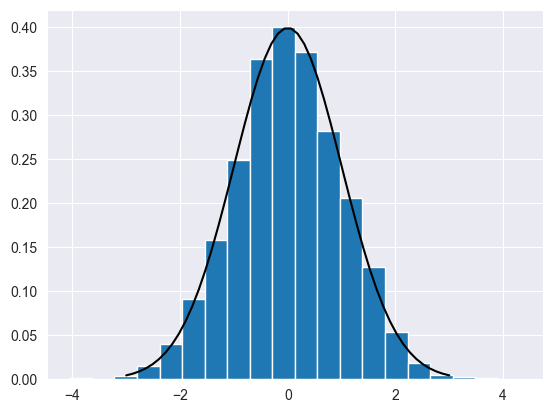
\includegraphics[width=0.4\textwidth]{histogram_of_sample4.png}
    
\end{frame}

%%%%
\begin{frame}[fragile]
\frametitle{Some miscellany about distributions in {\ttm numpy.random}}
\begin{itemize}
    \item Many other probability distributions are implemented in \ttt{numpy.random}. See \href{https://numpy.org/doc/2.1/reference/random/legacy.html#distributions}{this link} for information about them.
    
    %\pause
    \item There is a useful command to shuffle an array: randomizing the order of the entries in the array: \ttt{np.random.shuffle(the}\ct{_}\ttt{array)}.
    \begin{itemize}
        \item This changes \ttt{the}\ct{_}\ttt{array} in place.
    \end{itemize}

    %\pause
    \item Not only a 1d array; can get a matrix (or any order tensor) with entries sampled from the distribution by adjusting the \ttt{size} argument.
\end{itemize}

\begin{codeblock}

\begin{python}
# to get 30x2 matrix, entries from normal N(0,1)
np.random.normal(size=(30,2))
\end{python}

\end{codeblock}

\end{frame}

\section{Defining custom functions}


%%%%
\begin{frame}[fragile]
    \frametitle{How to define a custom function}
The basic structure for a definition of a custom function has four parts: the function name, a list of arguments it takes, the ``body'' of the function (what happens when it is called), and what it returns.

Like this:

\begin{codeblock}

    \begin{python}
    def function_name(argument1, argument2):
        # in this part is the body of the function
        return function_output
    \end{python}
    
    \end{codeblock}
    

\textbf{Example.} Here is a function that takes a 1d array as input. It makes a copy of it, but in reversed order.  Then it multiplies these together entry-wise, and any negative numbers obtained are replaced with 0. It then returns the resulting array of non-negative numbers.

\begin{codeblock}

\begin{python}
def my_function(v):
    reverse_v = v[::-1]
    multiplied = reverse_v * v
    zeros = np.zeros(len(v))
    return np.maximum(multiplied, zeros)
\end{python}

\end{codeblock}

\end{frame}

%%%%
\begin{frame}[fragile]
\frametitle{A custom function to help with a plot}
Say that I have 500 points in the plane. Maybe they are selected randomly in some way, such as 

\begin{codeblock}

\begin{python}[numbers=none]
p = np.random.uniform(-1, 1, size=(500,2))
\end{python}

\end{codeblock}

%\pause
Now, say that I want to plot them, coloring them dark blue if their dot product with the vector $(2,-2/3)$ is negative, and coloring them a \emph{salmon} color otherwise.

An efficient way to make the array that contains the colors, ordered as the points are?

\begin{codeblock}

\begin{python}
def coloring(array_of_points):
    ref_vector = np.array([2,-2/3])
    dotvalues = array_of_points@ref_vector
    colors = np.array(['darkblue' if v < 0 else 'salmon' for v in dotvalues])
    return colors
\end{python}

\end{codeblock}
\end{frame}

%%%%
\begin{frame}[fragile]
\frametitle{Additional arguments, default values, keyword arguments}

% or, def my_function(v, translate):
% or, def my_function(v, translate=2):

\begin{codeblock}

\begin{python}
def my_function(v, *, translate=2):
    reverse_v = v[::-1]
    multiplied = reverse_v * v + translate
    zeros = np.zeros(len(v))
    return np.maximum(multiplied, zeros)
\end{python}

\end{codeblock}

\end{frame}

\section{Importing data}

%%%%
\begin{frame}[fragile]
    \frametitle{Importing data with Pandas}
For this first example, we'll keep working with data very simple. 

Assumption: data is contained in a CSV file, representing a ``spreadsheet'' of values in columns.

\begin{enumerate}
    \item Import Pandas, command: \ttt{import pandas as pd}.
    \item If file is in same folder as your Jupyter notebook, and called \ttt{file1.csv}, then assign 
\end{enumerate}

\begin{codeblock}

\begin{python}[numbers=none]
df = pd.read_csv('file1.csv')
\end{python}

\end{codeblock}

The output, \ttt{df}, is a Pandas DataFrame. Assuming your CSV file had a first line with column headings (\ct{'column1', 'column2',}\ldots etc.), the values in the first column, type \ttt{df['column1']}.

A column of a dataframe has a method, \ct{.to_numpy()}, that converts it to a NumPy array.
\end{frame}

\end{document}